\chapter{Introdução}

As tecnologias computacionais relacionadas ao processamento de dados permitem uma melhor forma de manusear uma grande quantidade de informação. Se determinados processamentos fossem realizados manualmente, a quantidade de tempo necessária poderia inviabilizar a sua realização. Além disso, os eventuais resultados também poderiam estar sujeitos à erros de manipulação, os quais seriam difíceis de detectar. Considerado estas dificuldades, diversas áreas do cotidiano utilizam a tecnologia como uma aliada, por exemplo a Meteorologia, responsável pelo estudo do clima e das condições de tempo de uma determinada região.

Algumas das atribuições da Meteorologia compreendem o entendimento do estado presente da atmosfera, o chamado ``tempo meteorológico'', e a realização de previsões, a chamada ``previsão do tempo'' \cite{Vianello:Livro}. No caso do tempo meteorológico, se faz necessário medidas de diferentes variáveis como temperatura do ar, umidade relativa do ar, direção e velocidade do vento, precipitação, pressão atmosférica, radiação, dentre outras. Considerando o grande volume de dados comum a este domínio, é essencial que tecnologias, métodos e ferramentas auxiliem a realização dessas tarefas propostas.

Visando um melhor entendimento das questões meteorológicas de Manaus e da Amazônia, em março de 2010 foi fundado o \emph{Laboratório de Instrumentação Meteorológica} (LabInstru) da Escola Superior de Tecnologia (EST) da Universidade do Estado do Amazonas (UEA). Este laboratório dispõe, dentre outros, de uma estação meteorológica automática, localizada nas dependências da EST/UEA, sob as coordenadas \ang{03;05;32,5}S, \ang{60;00;59,69}W a 31 metros acima do nível do mar, na qual diversos sensores encontram-se instalados para medida e registros de diferentes variáveis meteorológicas \cite{Labinstru:EST}.

Além da manutenção da estação meteorológica, o LabInstru possui uma série de atribuições, tais como a organização dos dados coletados, disponibilização de dados para órgãos governamentais e para a sociedade, geração de boletins meteorológicos informativos, dentre outros. Atualmente, a maioria dessas atividades têm sido realizada de forma manual, um processo demorado e exaustivo, sujeito a erros e imprecisões e que requer mão de obra altamente especializada.

Para ilustrar o contexto considerado, um exemplo é apresentado na Figura \ref{fig:contexto}. Se um interessado desejar adquirir uma determinada informação, primeiramente deverá preencher um formulário online disponível no site do LabInstru e também entregar, presencialmente no próprio laboratório, o termo de compromisso adequado à sua solicitação devidamente preenchido (Etapa 1). Em seguida, a equipe do laboratório recebe uma notificação da solicitação (via e-mail) e inicia a preparação dos dados (Etapa 2). O passo seguinte consiste em consultar diferentes arquivos-texto resultantes da estação meteorológica a fim de precisar o intervalo de datas requerido (Etapa 3). A equipe irá agregar esses dados e utilizará aplicativos adequados para filtrar as variáveis meteorológicas requeridas pela solicitação (Etapa 4).

\begin{figure}[H]
	\centering
	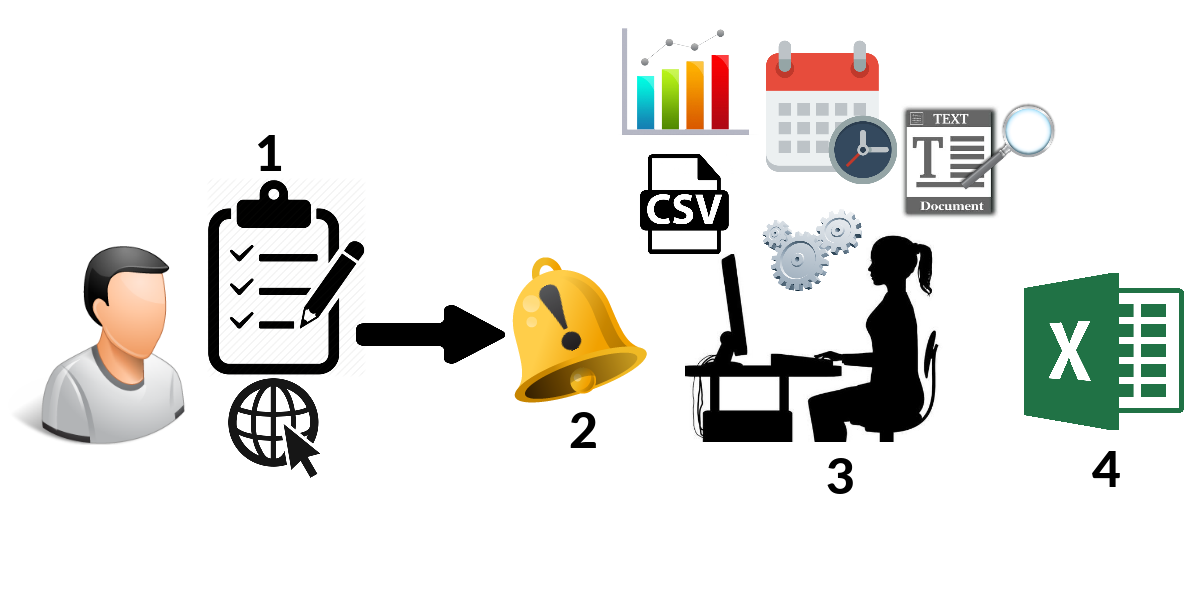
\includegraphics[width=0.6\textwidth]{./img/contexto.png}
	\caption{Contexto atual de uma das atividades realizadas pelo LabInstru. Fonte: Próprio Autor} 			\label{fig:contexto}
\end{figure}

Embora este exemplo ilustre o cenário atual do LabInstru, não compreende todas as dificuldades enfrentadas pela equipe do laboratório na realização de suas atribuições. Há que se mencionar as dificuldades na preparação de gráficos ilustrativos, na verificação da disponibilidade de dados, na geração de boletins meteorológicos, no controle e manuseio dos arquivos da estação meteorológica, dentre diversas outras.

Considerando este contexto, este trabalho de conclusão de curso teve por objetivo projetar e implementar uma plataforma web com vistas a colaborar na minimização das dificuldades mencionadas. E, como resultado, obteve-se a plataforma \emph{LabInstru Web}, desenvolvida na linguagem de programação Python, com o \emph{framework} Web2py e tecnologias como MySQL e Bootstrap, implantada na nuvem com o Google App Engine.  Esta plataforma é responsável por promover o armazenamento, gerenciamento, manutenção e disponibilização de dados da estação meteorológica automática da EST/UEA, administrada pelo LabInstru, fornecendo também uma visualização desses dados por meio de boletins meteorológicos.

\section{Objetivos}

O objetivo geral deste trabalho consistiu projetar e implementar uma plataforma web, para armazenamento, gerenciamento e disponibilização de dados de uma estação meteorológica automática. Para obtenção de sucesso no objetivo apresentado, fez-se necessário alcançar alguns objetivos específicos, a citar:

\begin{enumerate}
	\item Identificar e documentar as funcionalidades que a plataforma a ser desenvolvida deve prover;
	\item Elaborar protótipos de interface para validar as funcionalidades a serem desenvolvidas;
	\item Efetuar um levantamento das tecnologias para o desenvolvimento da plataforma web;
	\item Projetar e implementar a plataforma web;
	\item Implantar a plataforma web no LabInstru.
\end{enumerate}

\section{Justificativa}

O desenvolvimento de uma plataforma web para o LabInstru é importante por diversas razões. Primeiramente sabe-se que a forma como os dados meteorológicos são armazenados e as técnicas utilizadas para processamento influenciam diretamente na precisão e no tempo gasto para a realização de diversas tarefas. Assim, o desenvolvimento de uma plataforma para este domínio colabora diretamente na minimização destas dificuldades, visto que se propõe a  armazenar, gerenciar e disponibilizar os dados de maneira estruturada e automatizada.

Esta plataforma colabora de maneira direta com uma das atividades centrais do LabInstru, que compreende a organização dos dados coletados na estação instalada através do laboratório \cite{Labinstru:EST}. Há que se mencionar também que uma plataforma desta natureza favorece a divulgação dos dados meteorológicos produzidos. Estes são de interesse para pesquisadores de diversas áreas, para autoridades governamentais e também para a população em geral, como é amplamente visto na mídia.

Do ponto de vista da Engenharia de Computação, este trabalho de conclusão de curso também colabora com métodos e técnicas desta área do conhecimento aplicadas ao domínio da Meteorologia, auxiliando no desenvolvimento de uma plataforma que será usada em contexto real, por usuários reais e que irá colaborar para a manutenção de um laboratório de pesquisas de uma instituição pública de ensino superior, fomentando a realização de diversos outros trabalhos.

\section{Metodologia} \label{sec:metodologia}

A metodologia adotada para guiar as atividades deste trabalho de conclusão de curso é apresentada a seguir, a qual compreendeu a realização das seguintes atividades:

\begin{enumerate}[label=\textbf{Atividade \arabic*}.,leftmargin=*,labelindent=1em]
	\item Identificar um processo de desenvolvimento que possa acomodar as características do trabalho em questão, considerando que novos requisitos podem ser descobertos, que só há um desenvolvedor e que não deve haver \emph{overhead} na documentação das atividades;
	\item Estudo dos arquivos gerados pela estação meteorológica do LabInstru, pré-requisito para o entendimento de diversos requisitos;
	\item Efetuar a elicitação de requisitos funcionais e não funcionais referentes ao domínio do problema, construindo diagramas de caso de uso e documentando os requisitos descobertos apropriadamente;
	\item Utilizando uma ferramenta de \emph{mockups}, construir protótipos da interface gráfica que permitam validar junto ao cliente os requisitos identificados;
	\item Elencar uma ordem de implementação dos requisitos considerando as dependências entre os mesmos e o cronograma disponível do trabalho de conclusão de curso;
	\item Identificar tecnologias para o desenvolvimento da plataforma web, considerando \emph{frameworks} que possam ajudar nesta tarefa e também recursos que possam auxiliar no desenvolvimento do \emph{front-end}, permitindo a criação da interface gráfica com recursos que venham a prover uma boa usabilidade;
	\item Implementar os requisitos considerando a ordem anteriormente especificada;
	\item Escrever o trabalho de conclusão de curso I;
	\item Defesa do trabalho de conclusão de curso I;
	\item Implantar a plataforma web junto ao cliente, permitindo a utilização da mesma pelos pesquisadores do LabInstru. Avaliar a possibilidade de instalação em um servidor local ou hospedagem em um servidor externo;
	\item Escrever o trabalho de conclusão de curso II;
	\item Defesa do trabalho de conclusão de curso II.
\end{enumerate}

\section{Organização do Documento}

Para apresentar a solução proposta, este trabalho de conclusão de curso está organizado como segue. O Capítulo \ref{cap:fundamentacao} apresenta os conceitos essenciais que foram utilizados no desenvolvimento deste trabalho, incluindo o contexto da Estação Meteorológica da EST, o boletim meteorológico do LabInstru e conceitos da Meteorologia, tais como índice de calor e escala de Beaufort. O Capítulo \ref{cap:solucao} apresenta a solução proposta, contemplando desde uma visão geral da mesma, os artefatos de modelagem produzidos, protótipos e a versão executável da mesma implementada na linguagem de programação Python, com o \emph{framework} Web2py. Por fim, as considerações finais e sugestões de trabalhos futuros encontram-se descritos no Capítulo \ref{cap:consideracoes}.
